\documentclass{standalone}
% font set
\usepackage{ctex}
\usepackage{fontspec}
\usepackage[T1]{fontenc}
\usepackage[sc]{mathpazo}
\usepackage{anyfontsize}
\setmainfont{Source Serif 4}
\setsansfont{Source Sans 3}
\setmonofont{Menlo}
\setCJKmainfont[BoldFont=黑体-简 中等,ItalicFont=楷体-简 常规体]{宋体-简 常规体}

% colors
\usepackage[dvipsnames]{xcolor}
\definecolor{pku-red}{RGB}{139,0,18}
\usepackage{colortbl}
\newcommand{\light}[1]{\textcolor{Orchid}{#1}}
\newcommand{\contrastlight}[1]{\textcolor{TealBlue}{#1}}

% plots
\usepackage{tikz}
\usepackage{tikz-cd}
\usetikzlibrary{arrows}
\usetikzlibrary{arrows.meta,positioning,calc,3d}
\usetikzlibrary{automata}
\usepackage{pgfplots}
\pgfplotsset{compat=newest}
\tikzset{
    punkt/.style={
        rectangle,
        rounded corners,
        draw=black, very thick,
        minimum height=2em,
        inner sep=6pt,
        text centered,
        fill=gray!30
    }
}

% math package
\let\Bbbk\relax
\usepackage{amsmath}
\usepackage{mathrsfs}
\usepackage{amssymb}
\usepackage{amsfonts}
\usepackage{stmaryrd}
\usepackage{latexsym}
\usepackage{extarrows}
\SetSymbolFont{stmry}{bold}{U}{stmry}{m}{n}


\begin{document}
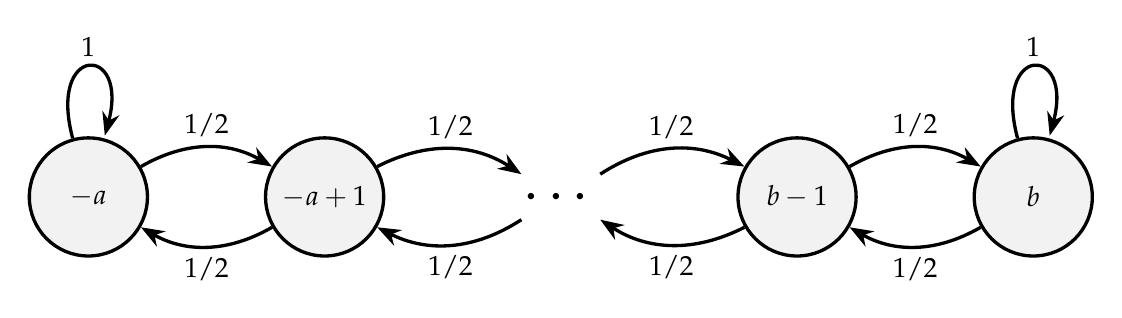
\begin{tikzpicture}[node distance=3cm, every state/.style={minimum size=1.5cm, very thick, fill=gray!10}, auto]

    % States
    \node[state] (A) {$-a$};
    \node[state] (A1) [right of=A] {$-a+1$};
    \node (dots) [right of=A1, scale=2] {$\dots$};  % Increased size of dots
    \node[state] (B1) [right of=dots] {$b-1$};
    \node[state] (B) [right of=B1] {$b$};

    % Transitions
    \path[->, >={Stealth},very thick] 
        % From A to A1
        (A1) edge[bend left] node[below] {1/2} (A)
        (A) edge[loop above] node {1} (A)
        (A) edge[bend left] node[above] {1/2} (A1)
        
        % From A1 to dots
        (A1) edge[bend left] node[above] {1/2} (dots)
        (dots) edge[bend left] node[below] {1/2} (A1)
        
        % From dots to B1
        (dots) edge[bend left] node[above] {1/2} (B1)
        (B1) edge[bend left] node[below] {1/2} (dots)
        
        % From B1 to B
        (B1) edge[bend left] node[above] {1/2} (B)
        (B) edge[loop above] node {1} (B)
        (B) edge[bend left] node[below] {1/2} (B1);

\end{tikzpicture}
\end{document}